% !TeX spellcheck = sl_SI
\documentclass{acm_proc_article-sp}
\usepackage[utf8]{inputenc}
\usepackage[slovene]{babel}
\usepackage{hyperref}

\graphicspath{ {slike/} }

\begin{document}

\title{Detekcija žaljivega besedila}
\subtitle{[Projekt pri predmetu Jezikovne tehnologije]}

\numberofauthors{6}

\author{
\alignauthor Andrej Hudrap\\
       \affaddr{Univerza v Mariboru, Fakulteta za računalništvo in informatiko, Smetanova ulica 17, 2000 Maribor, Slovenija}\\
       \email{andrej.hudrap\linebreak[0]@student\linebreak[0].um\linebreak[0].si}
\alignauthor Janez Krnc\\
       \affaddr{Univerza v Mariboru, Fakulteta za računalništvo in informatiko, Smetanova ulica 17, 2000 Maribor, Slovenija}\\
       \email{janez.krnc\linebreak[0]@student\linebreak[0].um\linebreak[0].si}
\alignauthor Žan Bezjak\\
       \affaddr{Univerza v Mariboru, Fakulteta za računalništvo in informatiko, Smetanova ulica 17, 2000 Maribor, Slovenija}\\
       \email{zan.bezjak\linebreak[0]@student\linebreak[0].um\linebreak[0].si}
\and
\alignauthor Klemen Berkovič\\
       \affaddr{Univerza v Mariboru, Fakulteta za računalništvo in informatiko, Smetanova ulica 17, 2000 Maribor, Slovenija}\\
       \email{klemen.berkovic\linebreak[0]@student\linebreak[0].um\linebreak[0].si}
}
\maketitle

\begin{abstract}
Razmah interneta in kasneje socialnih omrežij je v naše življenje prinesel mnogo tako pozitivnih, kot tudi negativnih posledic.
Ena izmed negativnih posledic je tudi razmah negativnega, sovražnega in žaljivega govora
Pri predmetu Jezikovne tehnologije se bomo znotraj projektne skupine osredotočili na detekcijo in zaznavo prav takšnih besedil oziroma delov besedil znotraj daljših sestavkov.
Kot že omenjeno se takšna vrsta besedil v veliki meri pojavlja na raznih socialnih omrežjih, forumih in ostalih mestih, kjer lahko uporabniki med seboj komunicirajo in zaradi tega bomo testna besedila jemali iz virov kot so Facebook, 24ur.com, slo-tech.com forumi.
Cilj našega projekta je spisati algoritem in program, ki bo sovražni in nezaželjen govor prepoznal ter besedilo prijavil administratorju, ki bi seveda lahko besedilo očistil žaljivih besed oziroma le-to v celoti odstranil.
\end{abstract}

\keywords{sovražni govor, žaljivi govor, žaljivke, zaznava žaljivk, detekcija žaljivk, preučevanje besedila}

\section{Uvod}
Razmah interneta in kasneje socialnih omrežij je v naše življenje prinesel mnogo tako pozitivnih, kot tudi negativnih posledic. 
Socialna omrežja nam omogočajo lažje ohranjanje stikov z oddaljenimi prijatelji in znanci in možnost hitre komunikacije z ostalimi uporabniki socialnega omrežja, vendar pa je prav zaradi odprtosti komunikacije prišlo do velikega razmaha negativnega, žaljivega in sovražnega govora.
Ljudje imamo različne poglede na svet in nemalokrat se pri izražanju nestrinjanja uporabijo neprimerne, žaljive besede. Žaljivi govor (tudi neprimerni govor) je opredeljen kot govor, pri katerem gre za žaljivo komunikacijo, ki je označena kot žaljivka, žaljiv izraz močnih čustev ali žaljivo govorjenje.
Prav tako so socialna omrežja postala raj za širjenje drugačnih pogledov na svet, kjer se nemalokrat med drugimi diskriminira različne manjšine in rase, kar spada pod sovražni govor.
Med sovražni govor spada ves govor, ki zmerja, žali, ustrahuje, spodbuja k nasilju, sovraštvu ali diskriminaciji. Jasno je, da so vse oblike negativno nastrojenega govora na socialnih omrežjih prepovedane, izziv pa je takšen govor avtomatsko razpoznati.
S podanim izzivom smo se s kolegi iz projektne skupine tudi (bolj ali manj) uspešno spopadli.

\section{Sorodna dela}
Analiza sentimenta ({\it ang. sentiment analsys}) oziroma analiza mnenj v besedilih ({\it ang. opinion minig}).
Ta tehnika se uporablja pri rudarjenju naravnega jezika.
V članku \cite{POI3:POI385} je uporabljena analiza sentimenta za boljšo detekcijo žaljivega govora na spletenih straneh.
V prej omenjenem članku je bilo veliko pozornosti namenjene pripravi učnih korpusov, ki so bili deljeni na več različnih tipov žaljitev.
Korpuse pred učenjem se prečistijo, tako da odstranijo odvečne besede in znake.
Pri čiščenju podatkov odstranijo tudi odvečne besede, ki ne vplivajo na pomen stavka.
Modele predvsem učijo na n-gramih, ki uporablja najmanj eno besedo in največ pet besed.
Prečiščene n-grame testirajo na SVM modelu, naključnem gozdu dreves ({\it Random Forest Decision Tree}), naivnem bayes modelu ({\it ang. Naive Bayes Classifier}) in ansambel klasifikatorjev, ki uporabljajo glasovanje za izbiranje izhodnega razreda.
V prej omenjenem članku je tudi opis metode priprave podatkov za klasifikacijo z uporabo metode kosa z besedami ({\it ang. bag of words}).

\section{Metode}
Množica komentarjev nad katerimi izvajamo učenje je v angleškem jeziku, saj smo si delo poizkušali olajšati s tem, da smo množico komentarjev pridobili s spleta ter jih klasificirali v razrede, ki smo jih preverjali. 
Preden smo komentarje poslali v algoritme za klasificiranje smo vseh 115 tisoč komentarjev naključno zamenjali med seboj. 
Za učno množico smo izbrali prvih 7 tisoč komentarjev, medtem ko smo naslednje 3 tisoč komentarjev uporabili za testno množico. Preostale komentarje smo zavrgli.

\subsection{Predprocesiranje komentarja}
Vsak prebran komentar smo pred samim učenjem oziroma testiranjem ustrezno obdelali. Komentar smo razdelili na dva dela, kjer nam je prvi del predstavljal tip komentarja (z 0 so označeni nežaljivi komentarji, medtem ko so z 1 označeni žaljivi in sovražni komentarji), drugi del pa je predstavljal samo vsebino komentarja. 

Obdelali smo tudi samo vsebino komentarja. V besedilu smo odstranili morebitne povezave, skoke v novo vrstico, tabulatorje, narekovaje, odvečne presledke in dvopičja ter celotno besedilo pretvorili v male črke. Poleg omenjenega preoblikovanja pa smo iz komentarja izločili tudi besede brez pomena ({\it ang. stopwords}), kot so any, these, which in drugo. Za na konec smo besedam še odstranili končnice.

V primeru učne množic smo tip komentarja shranjevali v polje, ki smo ga kasneje združili z značilkami, ki s v komentarju pojavljajo, ter nad združenim poljem izvedli algoritem. V primeru testnih množic smo tipe komentarja shranjevali zgolj zaradi preverjanja uspešnosti klasifikacije testne množice, s pomočjo katerih smo kasneje lahko izračunali natančnost klasifikacije v odstotkih.

\subsection{Bag-of-Words (BOW)}
Model vreče besed ({\it ang. Bag of words}) temelji na obdelavi značilk.
Iz besedila najprej z obdelavo slovarja vseh značilk, ki se pojavijo v vseh komentarjih, ter polja vseh komentarjev s pripadajočimi tipi pridobimo slovar s tipom komentarja in vektorjem pojavitve značilk za vse komentarje.
Za označitev značilk, ki se pojavijo v samem komentarju smo uporabili binarni model, kar pomeni, da smo za vsako značilko v slovarju, ki se pojavi v komentarju, na njeno mesto zapisali 1 oziroma za vsako značilko v slovarju, ki se v komentarju ne pojavi, smo na njeno mesto zapisali 0.

\subsection{Support Vector Machine (SVM)}
Modela za učenje {\tt SVM} ({\it ang. Support Vector Model}) nismo implementirali, temveč smo uporabili model {\tt SVM} iz knjižnice {\tt sklearn}.
Iz knjižnice {\tt sklearn} smo uporabili SVM model, ki se uporablja za klasifikacijo, ter ga v knjižnici {\tt sklearn} najdemo pod imenom {\tt SVC}.
Uporabljeni model se nadzorovano uči na podlagi podatkov za klasifickacijsko in regresijsko analizo.
Za učenje modelu lahko nastavimo tudi jedro, ki predstavlja algoritem za učenje.
V našem delu smo uporabili linearno jedro.
V sam model pošljemo podatke o tipih komentarja ter vektor s podatki o pojavitvi značilk v posameznem komentarju, model pa se na podlagi teh podatkov nauči in kasneje klasificira testne podatke.
Vec o modelu lahko najdete v članku \cite{Cortes1995}.

\subsection{Random Forest (RF)}
Metoda {\tt Random Forest} ({\it slov. Naključni gozdovi}) je ansambelska metoda, ki se na področju strojnega učenja in podatkovnega rudarjenja uporablja za klasifikacijo, regresijo ipd.
Metode nismo razvili sami, temveč smo jo uporabili iz knjižnice {\tt sklearn}.
Knjižnica {\tt sklearn} na ponuja dva tipa naključnih dreves.
Prvi tip naključnih dreves se uporablja pri regresji, ter jo najdemo v izbrani knjižnici pod imenom {\tt RandomForestRegressor}.
Drugi tip naključnih dreves se pa uporablja za klasifikacijo, ter jo najdemo v knjižnici {\tt sklearn} po imenom {\tt RandomForestClassifier}.
V našem delu smo uporabili metodo, ki podpira klasifikacijo.
Metoda deluje tako, da konstruira množico odločitvenih dreves pri učenju.
Vsako drevo uporablja različne učne podmnožice podatkov za učenje. Velikost učnih podmnožic so pri vseh naučenih drevesih enake.
Knjižnica {\tt sklearn} podpira izbiranje vzorcev učne možice na podlagi metode zamenjave, ki je uporabljena pri klasifikacijski metodi bagging.
Algoritem za učenje uporablja tudi tehniko povprečenja, s katero se skuša izogniti prekomernem prilagajanju učni množici.
Kot izhod dobimo razred, ki se pri klasifikaciji pri vseh odločitvenih drevesih najpogosteje pojavi.
V kolikor se izvaja regresija se izbere povprečna vrednost napovedi vseh odločitvenih dreves.
Več o samih naključnih gozdovih lahko izveste v člankih \cite{ho1998random, ho1995random}.

\subsection{Detekcija z n-grami}
N-gram je n dolga sekvenca enot, generirana iz podanega teksta.
Ponavadi na področju računalniške lingvistike in verjetnosti n-grame ločimo na besedne in znakovne n-grame. 
Stopnja n-grama ponavadi poteka od 1 do 5.
Kjer n-gram stopnje 1 imenujemo unigram, n-gram stopnje 2 bigram, n-gram stopnje 3 trigram in tako dalje. 
V naši metodi smo uporabljali izključno besedne n-grame.
Besedilo, ki smo ga želeli klasificirati smo razdelili na besedne n-grame, nakar smo le-te uporabili pri klasifikaciji besedila s pomočjo naučenega modela.
Metoda je odporna na nebesedne napake v besedilu.
V našem delu smo uporabili unigrame, bigrame in trigrame, ker napake najpogosteje popravimo ze na dolžini od 3 do 5 znakov.

\section{Meritve in rezultati}
\subsection{Vrednotenje meritev}
Na področju strojnega učenja in posebej problem statistične klasifikacije se za vrednotenje rezultatov uporablja kontingenčna matrika({\it ang. confusion matrix}), znana tudi kot matrika napake.
Kontingenčna matrika je tabelarična predstavitev podatkov, ki omogočajo vizualizacijo algoritmom za napovedovanje.

\begin{figure}[!h]
	\centering
	\caption{Primer mnozice rezultatov klasifikatorja} \label{mnozicaZadetkov}
	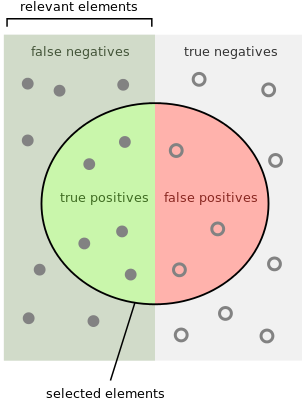
\includegraphics[scale=0.45]{Precisionrecall}
\end{figure}

Slika \ref{mnozicaZadetkov} prikazuje množico posameznikov, ki so označeni z majhnimi polnimi in praznimi krogi.
Na sliki \ref{mnozicaZadetkov} je prikazan tudi večji krog, ki pa predstavlja vrednosti klasifikacije z izbranim klasifikatorjem.
Kvaliteto klasifikatorja ocenjujemo na podlagi velikega kroga.
Več kot je pravilno klasificiranih primerkov v razredu, ter manj kot je napačno klasificiranih primerkov, boljši je izbrani klasifikator.
Na sliki \ref{mnozicaZadetkov} imamo prikazane štiri tipe frekvenčnih podatkov, ki nastopajo v kontigenčni matriki. 
Tabela \ref{defConfmatrix} prikazuje štiri tipe frekvenčnih podatkov, ki so elementi kontingenčne matrike.

\begin{table}[h!]
	\centering
	\caption{Pomeni spremenljivk v formulah} \label{defConfmatrix}
	\begin{tabular}{|c|c|} 
		\hline
		\textbf{Kratica} & \textbf{Pomen} \\ \hline
		$ tp $ & rue positive (pravilno klasificirani 1) \\ \hline
		$ fp $ & false positive (v resnici 0, klasificirani kot 1) \\ \hline
		$ tn $ & true negative (pravilno klasificirani 0) \\ \hline
		$ fn $ & false negative (v resnici 1, klasificrani kot 0) \\ \hline
		$ p $ & all positive (vsi ki spadajo v 1) \\ \hline
		$ n $ & all negative (vsi ki spadajo v 0) \\ \hline
	\end{tabular}
\end{table}

S pomočjo kontingenčna matrike lahko pridobimo podatke o preciznosti, priklicu, natančnosti in vrednosti funkcije $ F1 $.

$$ precision = \frac{tp}{tp + fp} $$
$$ recall = \frac{tp}{tp + fn} $$
$$ accuracy = \frac{tp + tn}{tp + tn + fp + fn} $$
$$ f1 = 2 \cdot \frac{precision \cdot recall}{precision + recall} $$
\subsection{Rezultati}
Pri vseh metodah smo za učenje uporabili uni-grame, bi-grame in tri-grame.

\subsubsection{SVM}
\begin{table}[h!]
	\centering
	\caption{Meritve za model SVM}
	\begin{tabular}{|c|c|c|c|c|}
		\hline
		\textbf{Razred} & \textbf{Natančnost} & \textbf{Odpoklic} & \textbf{F1} & \textbf{Podpora} \\ \hline
		Ni žaljivo & 0.67 & 0.79 & 0.73 & 501 \\ \hline
		Je žaljivo & 0.75 & 0.61 & 0.67 & 499 \\ \hline \hline
		povprečje & 0.71 & 0.70 & 0.70 & 1000 \\ \hline
	\end{tabular}
\end{table}
Natančnost modela 70.3\% (703/1000).

\subsubsection{Random forest}
\begin{table}[h!]
	\centering
	\caption{Meritve za model Random forest}
	\begin{tabular}{|c|c|c|c|c|}
		\hline
		\textbf{Razred} & \textbf{Natančnost} & \textbf{Odpoklic} & \textbf{F1} & \textbf{Podpora} \\ \hline
		Ni žaljivo & 0.58 & 0.72 & 0.65 & 501 \\ \hline
		Je žaljivo & 0.63 & 0.48 & 0.55 & 499 \\ \hline \hline
		povprečje & 0.61 & 0.60 & 0.60 & 1000 \\ \hline
	\end{tabular}
\end{table}
Natančnost modela 60.5\% (605/1000).

\subsection{Interpolacija rezultatov}
TODO

\section{Zaključek}
TODO

\bibliographystyle{abbrv}
\bibliography{sigproc} 

\end{document}}